\chapter{}
\label{app:d}

\[
\text{For a circle centered in } (x_c, y_c) \text{ with radius } r \text{ and } N \text{ pegs}:
\]

\[
\begin{aligned}
x_k &= x_c + r \cdot \cos\left( \frac{2\pi k}{N} \right), \\
y_k &= y_c + r \cdot \sin\left( \frac{2\pi k}{N} \right),
\end{aligned}
\quad \text{for } k = 0, 1, 2, \dots, N - 1
\]

\[
\text{The nearest first two points are:}
\]

\[
p0 = (r\cos(0), r\sin(0)) = (r, 0),
\]
\[
p1 = (r\cos(\frac{2\pi}{N}), r\sin(\frac{2\pi}{N}))
\]

\[\text{The Manhattan distance } d \text{ between two adjacent pegs is:}\]

\[
\begin{aligned}
d &= \left| x_1 - x_0 \right| + \left| y_1 - y_0 \right| \\
  &= \left| p1_x - p0_x \right| + \left| p1_y - p0_y \right| \\
  &= \left| r\cos\left(\frac{2\pi}{N}\right) - r \right| + \left| r\sin\left(\frac{2\pi}{N}\right) \right| \\
  &= r\left( \left| \cos\left(\frac{2\pi}{N}\right) - 1 \right| + \left| \sin\left(\frac{2\pi}{N}\right) \right| \right) \\
  &= \frac{w}{2} \left( \left| \cos\left(\frac{2\pi}{N}\right) - 1 \right| + \left| \sin\left(\frac{2\pi}{N}\right) \right| \right), \quad \text{where } r = \frac{w}{2}
\end{aligned}
\]

\chapter{}
\label{app:greedy}

\begin{algorithm}
\caption{Greedy Algorithm}
\begin{algorithmic}[1]
\State $k \gets \text{number of lines to select (input)}$ \\

\While{$k > 0$}
    \State $E$ \Comment{the lines not yet drawn, selected using one of the two heuristics. \(E\) is a matrix containing canonical vectors}
    \State $j \gets 0$ \Comment{index of the candidate line that reduces the error the most} \\
    \For{$i = 1$ to $n$}
        \If{$\left\| A(x + E_j) - b \right\| < \left\| A (x + E_i) - b \right\|$}
            \State $j \gets i$
        \EndIf
    \EndFor \\

    \If{$\left\| A(x + E_j) - b \right\| >= \left\| Ax - b \right\|$}
        \State \textbf{break}
    \EndIf \\

    \State $x \gets x + E_j$
    \State $k \gets k - 1$
\EndWhile
\end{algorithmic}
\end{algorithm}

\chapter{}
\label{app:omp}

\begin{algorithm}
\caption{Orthogonal Matching Pursuit (OMP) Algorithm}
\begin{algorithmic}[1]
\State $k \gets \text{number of lines to select (input)}$ \\

\While{$k > 0$}
    \State $j \gets argmax(A^Tb)$ \Comment{index of the column vector that reduces the error the most} \\

    \If{$\left\| A(x + E_j) - b \right\| >= \left\| Ax - b \right\|$}
        \State \textbf{break}
    \EndIf \\

    \State $b \gets b - A_j$ \Comment{where $A_j$ is the column $j$ of $A$}
    \State $x \gets x + E_j$
    \State $k \gets k - 1$
\EndWhile
\end{algorithmic}
\end{algorithm}

\chapter{}
\label{app:radon_quantitative}

\begin{figure}[H]
    \centering
    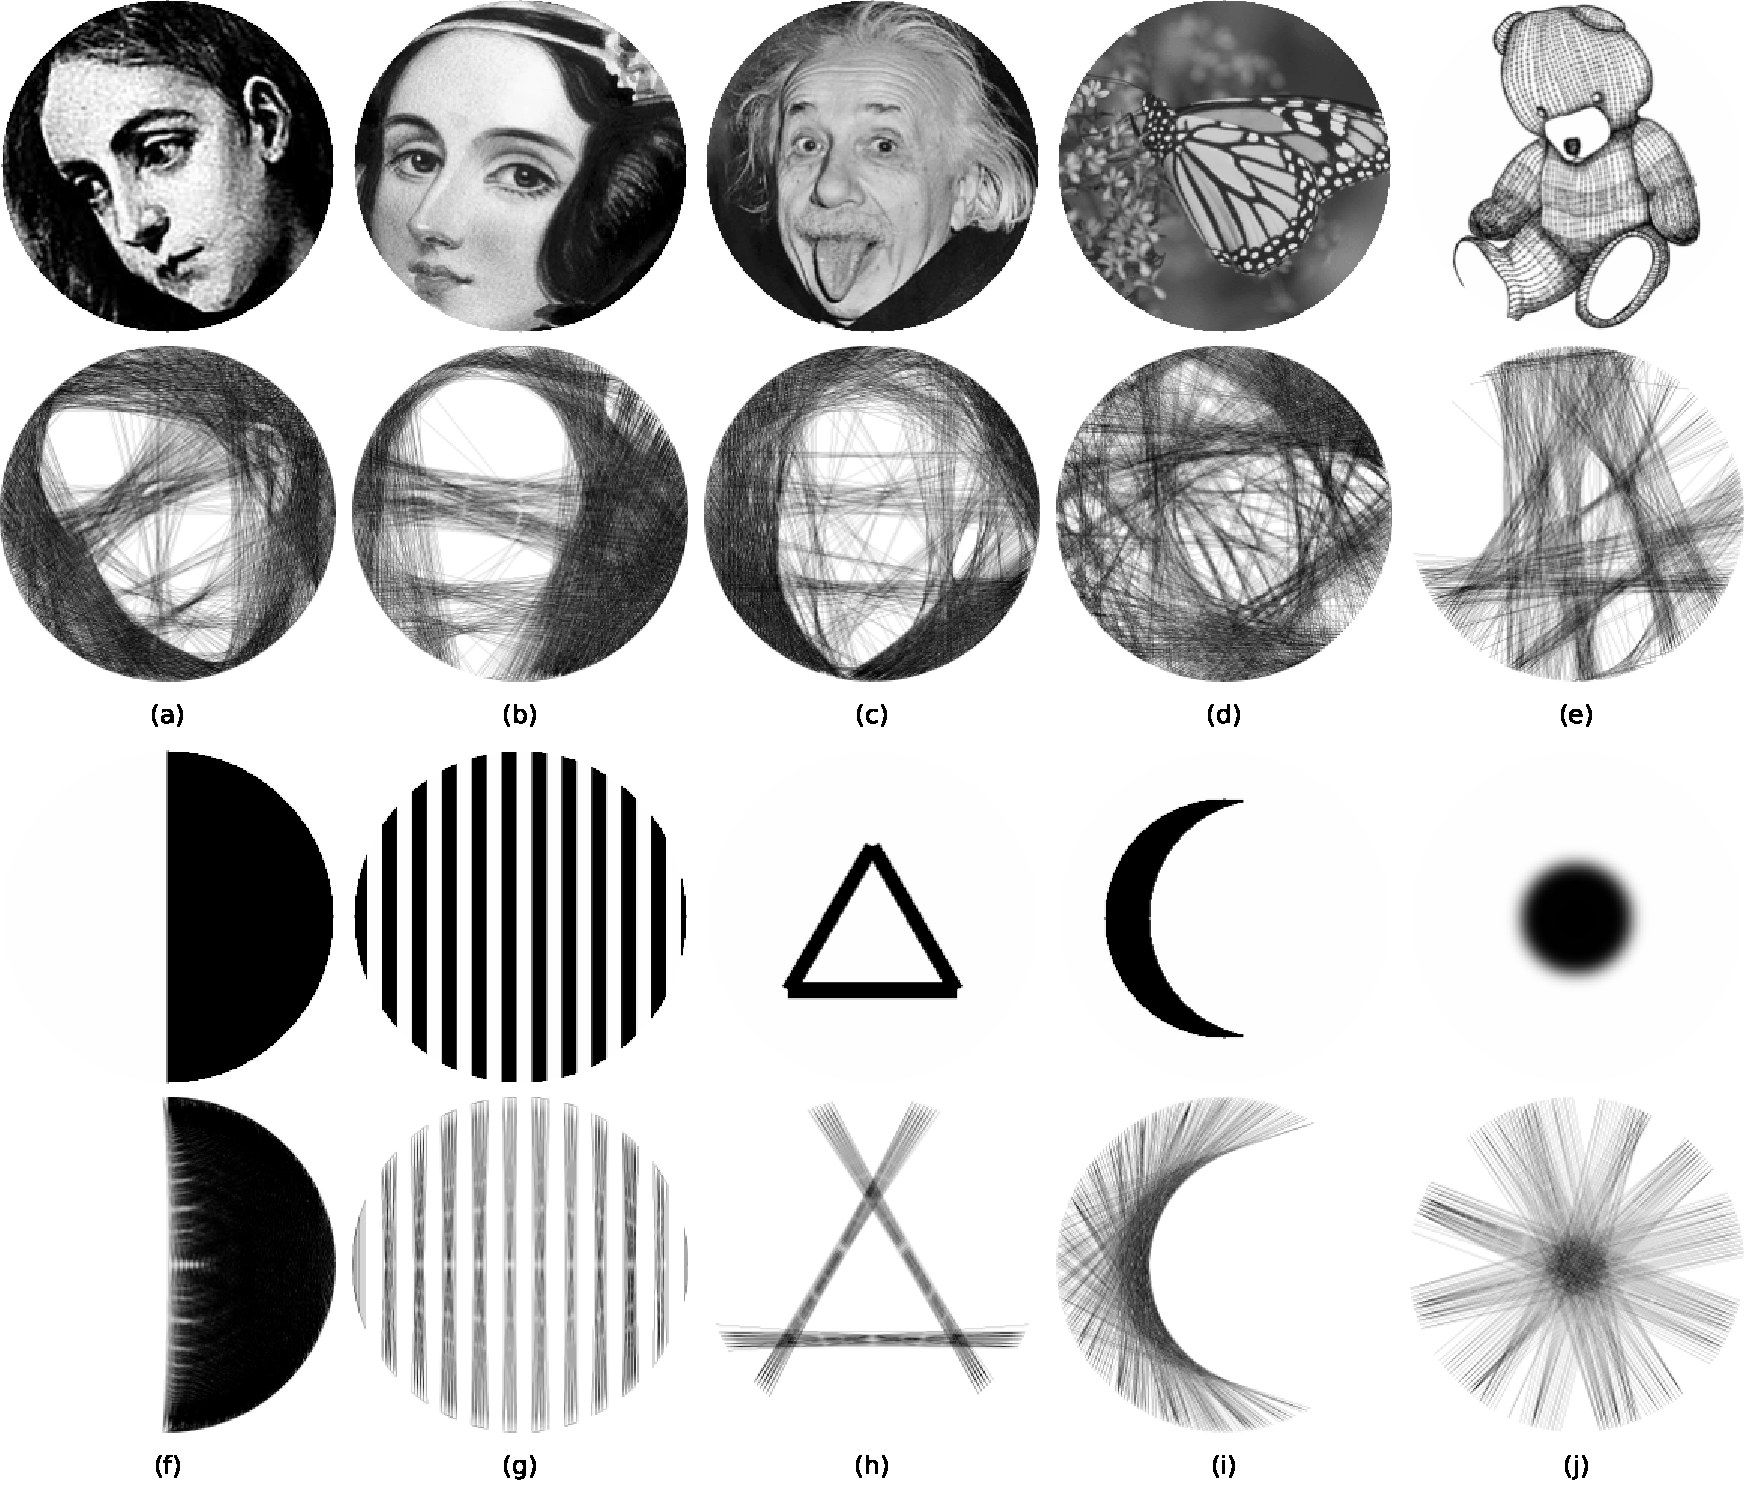
\includegraphics[width=\linewidth]{images/radon/radon_quantitative_test.pdf}
    \caption{Comparative analysis of reconstruction results using the Radon solver. The top image shows the input target image, while the bottom image displays the corresponding reconstruction. The solver was configured with 256 pegs and a patience factor of 10.}
    \label{fig:radon_quantitative}
\end{figure}

\begin{figure}[H]
    \centering
    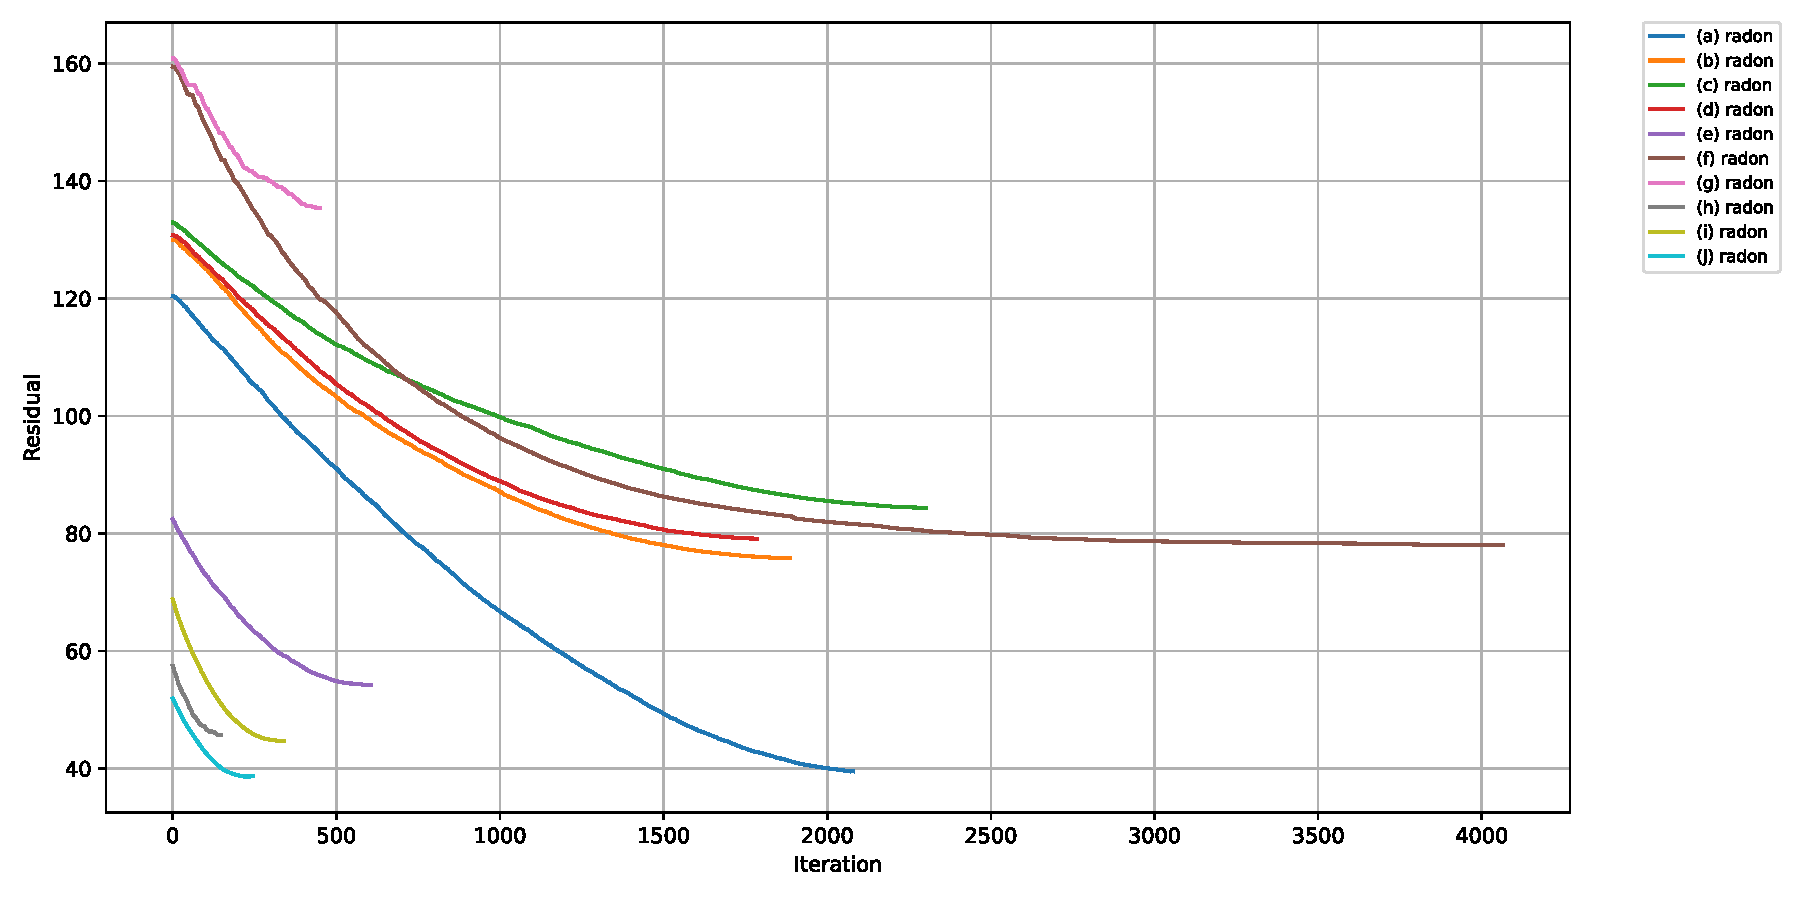
\includegraphics[width=\linewidth]{images/radon/residual_history.pdf}
    \caption{Residual error over iterations for each Radon solver.}
    \label{fig:radon_norm_error}
\end{figure}

\begin{table}[!ht]
\centering
\caption{Computation Time, Peak Memory Usage, RMS and number of Selected Lines for each Radon solver.}
\begin{tabularx}{\textwidth}{l C C C C}
\toprule
\textbf{Label} & \textbf{Computation Time (s)} & \textbf{Peak Memory Usage (MB)} & \textbf{RMS} & \textbf{Selected Lines} \\
\midrule
(a) & 2430            & 868.132            & 0.2557            & 1795 \\
(b) & 2406            & 868.131            & 0.1912            & 1579 \\
(c) & 2741            & 868.131            & 0.1906            & 1822 \\
(d) & 2159            & 868.131            & 0.2232            & 1538 \\
(e) &  821            & 868.131            & 0.2505            &  539 \\
(f) & 1216            & 868.132            & \textbf{0.1283}   & \textbf{2449} \\
(g) &  639            & 868.131            & 0.5104            &  312 \\
(h) &  \textbf{272}   & 868.131            & 0.2234            &   86 \\
(i) &  471            & 868.131            & 0.2266            &  323 \\
(j) &  375            & 868.131            & 0.2795            &  242 \\
\bottomrule
\end{tabularx}
\end{table}